\section*{Estimadores de Bayes}
\begin{frame}{Estimadores de Bayes}
 \begin{itemize}
  \item  Estimador e estimativa;
  \item Função de perda;
  \item Estimador de Bayes;
  \item Consistência do estimador de Bayes;
  \item Estimador de Bayes para grandes amostras;
  \item Limitações.
 \end{itemize}
\end{frame}


\begin{frame}{Prioris impróprias}
 \begin{defn}[Priori imprópria]
 Seja $\xi : \Lambda \to (0, \infty)$, $\Omega \subseteq \Lambda$, uma função tal que $\int_{\Omega} \xi(\theta)\,d\theta = \infty$.
 Se utilizamos $\xi$ como uma p.d.f. para $\theta$, dizemos que $\xi$ é uma~\textbf{priori imprópria} para $\theta$.
 \end{defn}
\begin{exemplo}[Priori imprópria para a taxa de uma Poisson]
   Suponha que $\rs$ formam uma amostra aleatória com distribuição Poisson com taxa $\theta > 0$, desconhecida.
   Desta vez, fazemos a escolha de hiperparâmetros $\alpha = \beta = 0$, o que leva a 
   \begin{equation*}
    \xi(\theta) = \frac{1}{\theta}.
   \end{equation*}
A posteriori passa a ser 
  \begin{equation*}
   \xi(\theta \mid \boldsymbol{x}) = \frac{ n^{S} }{\Gamma(S)} \theta^{n-1} e^{-S\theta},
  \end{equation*}
   onde $S = \sum_{i=1}^n x_i$.
\end{exemplo}
\end{frame}

\begin{frame}{Estimadores (de Bayes)}

\begin{defn}[Estimador]
Sejam $\rs$ variáveis aleatórias com distribuição conjunta indexada por $\theta$.
Um~\textbf{estimador} de $\theta$ é qualquer função real $\delta: \rs \to \mathbb{R}^d$, $d\geq 1$. 
\end{defn}
\begin{defn}[Estimativa]
Dizemos que o valor de $\delta$ avaliado nas realizações de $\rs$, $\boldsymbol x = \{ x_1, x_2, \ldots, x_n\}$,  $\delta(\boldsymbol{x})$ é uma~\textbf{estimativa} de $\theta$.
\end{defn}

\begin{defn}[Função de perda]
Uma função de perda é uma função real em duas variáveis 
\[ L : \Omega \times \mathbb{R}^d \to \mathbb{R}, \]
em que dizemos que o estatístico~\underline{perde} $L(\theta, a)$ se o parâmetro vale $\theta$ e a estimativa dada vale $a$.
\end{defn} 
\end{frame}

\begin{frame}{Funções de perda e estimadores bayesianos}
Exemplos de funções de perda são $L(\theta, a) = (\theta-a)^2$ e $L(\theta, a) = |\theta-a|$.
\begin{obs}[Perda esperada~\textit{a priori}]
Se escolhemos uma priori $\xi(\theta)$, nossa perda esperada,~\textbf{antes} de observar os dados é
\begin{equation*}
 E_\xi[L(\theta, a)] = \int_{\Omega} L(\theta, a)\xi(\theta)\,d\theta.
\end{equation*}
Vemos então que a escolha da distribuição~\textit{a priori} está inextrincavelmente ligada à função de perda.
\end{obs}
\end{frame}

\begin{frame}{Estimador de Bayes}
 \begin{defn}[Estimador de Bayes]
  Considere a perda esperada~\textit{a posteriori}:
  \begin{equation*}
   E_{\theta \mid \boldsymbol{x}}\left[L(\theta, a) \right] = E[L(\theta, a) \mid \boldsymbol{x}] = \int_{\Omega} L(\theta, a)\xi(\theta \mid \boldsymbol{x})\, d\theta. 
  \end{equation*}
Dizemos que $\delta^\ast$ é um~\textbf{estimador de Bayes} se, para toda realização $\boldsymbol{X} = \boldsymbol{x}$,
\begin{equation*}
 E[L(\theta, \delta^\ast(\boldsymbol{x}) ) \mid \boldsymbol{x}] = \min_{a \in \mathcal{A}}   E[L(\theta, a) \mid \boldsymbol{x}].
\end{equation*}
 \end{defn}
\begin{itemize}
 \item Em outras palavras, um estimador de Bayes é uma função real dos dados que minimiza a perda esperada com respeito à posteriori dos parâmetros.
\end{itemize} 
\end{frame}

\begin{frame}{Estimador de Bayes sob perda quadrática}
Suponha que a função de perda seja 
\[ L(\theta, \delta^\ast) =  (\theta-\delta^\ast)^2. \]
Dizemos que a função de perda é~\textbf{quadrática}.
Temos o seguinte resultado:
 \begin{theo}[$\delta^\ast$ sob perda quadrática]
  \label{thm:posterior_mean_quadratic}
  (De Groot, Corolário 7.4.1)
  
  Seja $\theta$ um parâmetro tomando valores reais.
  Sob perda quadrática,
  $$\delta^\ast(\boldsymbol{x}) = E[\theta | \boldsymbol{X} = \boldsymbol{x}] = \int_{\Omega} \theta \xi(\theta \mid \boldsymbol{x} ) \,d\theta.$$
 \end{theo}
 \textbf{Prova:} Escrever a perda esperada~\textit{a posteriori} explicitamente, usar a lei de esperanças e minimizar a expressão resultante com respeito ao estimador (ex. diferenciar e igualar a derivada a zero).
\end{frame}

\begin{frame}{Estimador de Bayes sob perda absoluta}
 \begin{theo}[$\delta^\ast$ sob perda absoluta]
  \label{thm:posterior_median_absolute}
  (De Groot, Corolário 7.4.2)
  
  Suponha que a função de perda é dada por  
\[ L(\theta, \delta^\ast) =  |\theta-\delta^\ast|. \]
Dizemos que a função de perda é~\textbf{absoluta}.
  
  Seja $\theta$ um parâmetro tomando valores na reta.
  Sob perda absoluta, $\delta^\ast(\boldsymbol{x})$ é a~\textbf{mediana}~\textit{a posteriori}, isto é,
  $$\int_{-\infty}^{\delta^\ast(\boldsymbol{x})}\xi(\theta \mid \boldsymbol{x} ) \,d\theta = \frac{1}{2}.$$
 \end{theo}
 \textbf{Prova:} Decompor a perda esperada em duas integrais de funções não-negativas utilizando as propriedades da função valor absoluto e aplicar a regra de Leibnitz duas vezes para encontrar o ponto de mínimo.
\end{frame}


\begin{frame}{O estimador de Bayes em grandes amostras}
\begin{itemize}
 \item Sob condições brandas de regularidade, à medida que o tamanho de amostra cresce, a influência da priori diminui.
\end{itemize}

\begin{exemplo}[Proporção de itens defeituosos]
Suponha que estamos interessados na proporção $\theta$ de itens defeituosos em uma linha de produção.
Suponha ainda que
\begin{itemize}
 \item Priori 1: $\xi_1(\theta) = 1$, $0 < \theta < 1$;
 \item Priori 2: $\xi_2(\theta) = 2(1-\theta)$, $0 < \theta < 1$;
 \item Dados: de $n = 100$ itens observados, $y = 10$ apresentaram defeito.
\end{itemize}

Perguntas:
\begin{itemize}
 \item $\bar{x}_n$ = ?
 \item $E_1[\theta \mid \boldsymbol{x}] = \int_{0}^1 \theta \xi_1(\theta \mid \boldsymbol{x})\,d\theta$ = ?
%  \item $E_2[\theta \mid \boldsymbol{x}] = \int_{0}^1 \theta \xi_2(\theta \mid \boldsymbol{x})\,d\theta$ = ?
\end{itemize} 
\end{exemplo}
\end{frame}

\begin{frame}{Proporção de itens defeituosos: prioris e posterioris}
Ver também exemplo 7.3.3 de De Groot.
\begin{figure}[!ht]
\label{fig:defect_items}
\begin{center}
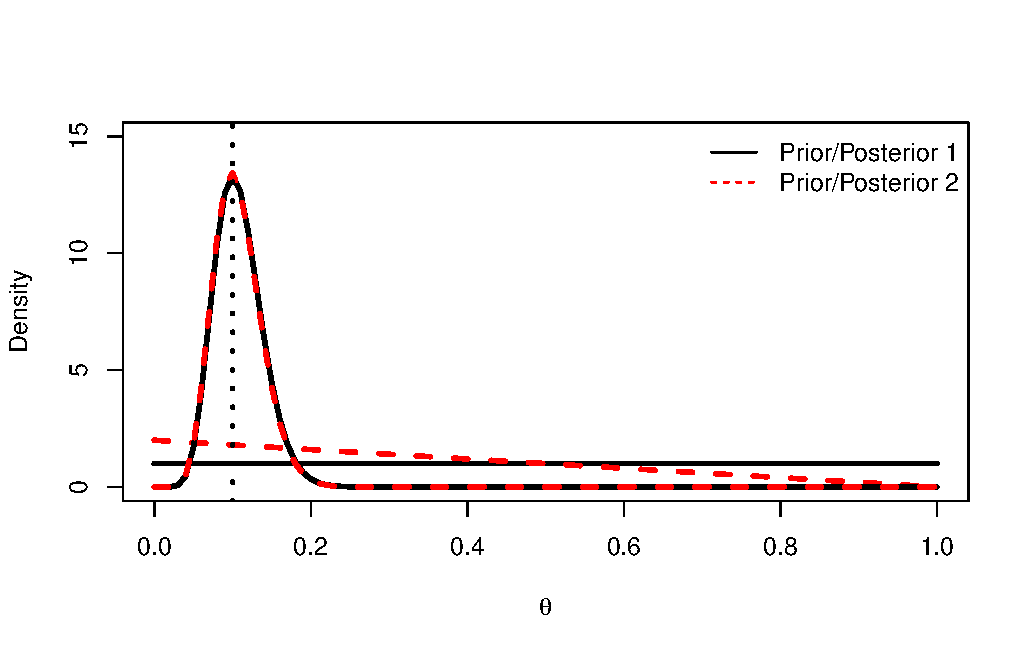
\includegraphics[scale=0.65]{figures/defeituosos.pdf} 
\end{center} 
\end{figure} 
\end{frame}


\begin{frame}{Consistência do estimador de Bayes}
\begin{defn}[Estimador consistente]
Seja $\delta_1, \delta_2, \ldots, \delta_n$ uma sequência de estimadores de $\theta$.
Se quando $n \to \infty$ a sequência converge para $\theta$, dizemos que esta é uma sequência consistente de estimadores.
\end{defn} 

\begin{obs}[A média amostral é consistente para o caso Bernoulli]
 Se $\rs$ são i.i.d. Bernoulli com parâmetro $\theta$ condicional a $\theta$, temos pela LGN: $\bar{X}_n \xrightarrow{\text{p}} \theta$.
\end{obs}

\begin{obs}[O estimador de Bayes é consistente para o caso Bernoulli]
 Para $\alpha > 0$ e $\beta > 0$ fixos, a média~\textit{a posteriori} vale
 $$\delta^\ast(\boldsymbol{x}) = E[\theta \mid \boldsymbol{x}] = \frac{\alpha + y}{\alpha + \beta + n}, $$
 onde $ y = \sum_{i=1}^n x_i$.
 É fácil ver que $\delta^\ast(\boldsymbol{x}) \xrightarrow{\text{p}} \bar{x}_n \xrightarrow{\text{p}} \theta$.
\end{obs}


\end{frame}

\begin{frame}{O que aprendemos?}
\begin{itemize}
 \item[\faLightbulbO] Estimador;
 
  ``Um estimador é qualquer função real dos dados''
  
 \item[\faLightbulbO] Função de perda;
 
  ``Uma função real que quantifica a perda incorrida por uma estimativa incorreta'' 
 
 \item[\faLightbulbO] Estimador de Bayes;
 
  ``Um estimador que minimiza a perda esperada~\textit{a posteriori}''
  
 \item[\faLightbulbO] Propriedades e limitações do estimador de Bayes;
 
  ``À medida que o tamanho da amostra cresce, o estimador se aproxima do valor verdadeiro, a influência da priori diminui, mas precisamos sempre de uma função de perda bem especificada'' 
 \end{itemize}
 
 \end{frame}

\begin{frame}{Leitura recomendada}
\begin{itemize}
 \item[\faBook] De Groot seção 7.4;
 \item[\faBook] $^\ast$ Casella \& Berger, seção 7.2.3.
 \item {\large\textbf{Exercícios recomendados}}
 \begin{itemize}
  \item[\faBookmark] De Groot, seção 7.4: exercícios 2, 4, 7, 11 e 14.
  \end{itemize}
 \end{itemize} 
\end{frame}


